\documentclass[10pt, twocolumn]{article}
\usepackage{amsmath,amssymb,amsfonts}
\usepackage{graphicx}
\usepackage{subcaption}
\usepackage{float}
\usepackage{url}
\usepackage{geometry}

\geometry{
  top=0.5in,
  left=1in,
  right=1in,
  bottom=1in
}

\setlength{\parindent}{0pt}
\setlength{\parskip}{1pt}

\renewenvironment{abstract}
{
  \centering\normalfont
}
{}

\setlength{\textfloatsep}{1pt}
\setlength{\intextsep}{1pt}

\begin{document}

\title{Pursuit Curves: An Exploration of A Differential Game}

\author{Tebe Nigrelli, Tommaso Ferracina}
\date{\today}

\twocolumn[
  \maketitle
  \begin{center}
    \begin{minipage}{0.9\textwidth}
      \begin{abstract}
        We study a variation of the Homicidal Chauffeur Problem in $\mathbb{R}^2$, a differential game involving two agents: an agile prey and a fast predator. We set the strategy of the prey to right-angle acceleration, whereas the predator uses a Proportional Navigation (PN) strategy. We simulate the trajectories using Runge-Kutta 4 integration, leveraging the Python Numba library for computational efficiency. We analyse individual trajectories using summary statistics and Fourier decomposition via the Discrete Cosine Transform. Finally, we explore a large phase space, varying predator speed and prey acceleration and identify regions of behavior corresponding to different capture dynamics. Our results highlight distinct strategy regimes and the expressivity of summary statistics to characterize pursuit-evasion games.
      \end{abstract}
    \end{minipage}
  \end{center}
]
\section{Introduction}
{\setlength{\parskip}{0pt}
The Homicidal Chauffeur Problem, first formulated by Rufus Isaacs in his 1951 paper "Games of Pursuit", is a classical pursuit-evasion differential game. It models the dynamics between a pursuer $P$, and an evader $E$, constrained to move in a plane. The pursuer is faster $v_2 > v_1$ but subject to a minimum turning radius, while the evader can maneuver freely. Capture is defined as the moment when the evader enters the pursuer's, with the capture time serving as the game's payoff.}

The relevance of this framework extends from missile guidance to predator-prey interactions in biology. Inspired by Isaac's model, we study a 2D variant where the pursuer uses Proportional Navigation (PN) while the evader executes right-angle evasive maneuvers. Our investigation focuses on deterministic strategies and analyzes their outcomes both dynamically and through the Discrete Cosine Transform.

\subsection{General Setting}
At initialization, we set the prey to its maximum speed, while varying the initial direction (bearing). Since the proportional navigation algorithm requires the predator to be moving at initialization, we set it to move at maximum speed towards the prey. Finally, we set initial acceleration to zero and place the two agents at a high distance from each other.

\[
  \begin{array}{l}
    \left\{
      \begin{aligned}
        x(0) &=
        \begin{pmatrix} 10 \\ 0
        \end{pmatrix} \\
        y(0) &=
        \begin{pmatrix} 0 \\ 0
        \end{pmatrix}
      \end{aligned}
      \right.
    \end{array}
    \begin{array}{l}
      \left\{
        \begin{aligned}
          \dot{x}(0) &=
          \begin{bmatrix}
            \cos\theta & -\sin\theta \\
            \sin\theta & \cos\theta
          \end{bmatrix}
          \begin{pmatrix}
            v^x_{\text{max}} \\
            0
          \end{pmatrix} \\
          \dot{y}(0) &=
          \begin{pmatrix} v^y_{\text{max}} \\ 0
          \end{pmatrix}
        \end{aligned}
        \right.
      \end{array}
    \]

    As a data object, we use a \texttt{state} numpy tensor to precompute the trajectory, before plotting it in its entirety. For ease of implementation, in the RK4 computation the tensor is unpacked into 2D arrays, before being repacked at the end of the computation. Written formally, the simulation produces the trajectory tuple $(x,y)(t)\in \mathbb{R}^2 \times \mathbb{R}^2 \times \mathbb{R}^+$.

    On a sidenote, it should be noted that the equations of motion for both prey (x) and predator (y) are defined solely by their acceleration, therefore position and velocity are actually redundant. In the simulation, we store all derivatives to compute and display the final metrics more easily.

    \subsubsection{Prey Behaviour}
    In the simulation, we fully characterise the behaviour of the prey by setting its acceleration vector to the direction orthogonal to the predator-prey vector. Acceleration is only altered when the predator gets within the prey's reaction distance. As a result, acceleration is maintained until the predator returns close enough to the prey. Consequently, the prey's acceleration is always fully dependent on the relative positions of the agents during the last `near miss' event.

    \[
      \begin{aligned}
        \Delta r &= x(t) - y(t), \\
        \Delta v &= \dot{x}(t) - \dot{y}(t), \\
        \ddot{x}(t) &=
        \begin{cases}
          - a_x^{\max}
          \begin{bmatrix}
            0 & -1 \\
            1 & 0
          \end{bmatrix}
          \hat{r}(t), & \|\Delta r\| < R_{\mathrm{react}}, \\[1.2em]
          \ddot{x}\bigl(t^*_{\mathrm{last\,react}}\bigr), & \|\Delta r\| \ge R_{\mathrm{react}}.
        \end{cases}
      \end{aligned}
    \]
    \subsubsection{Predator Behavior}
    We model the predator through the "Proportional Navigation" algorithm, which induces lateral acceleration proportional to the rate of change of the Line Of Sight (LOS) of the target. Through this mechanism, the velocity vector rotates constantly, up to interception. The predator thus accelerates in a direction orthogonal to the LOS vector, with strength proportional to the rate at which the angle between it and the prey changes.
    \[
      \begin{aligned}
        \hat r(t) &= \frac{\Delta r}{\|\Delta r\|},
        &\quad &\mathrm{unit\ LOS};\\
        \dot\lambda(t) &= \frac{\Delta r_x\,\Delta v_y - \Delta r_y\,\Delta v_x}{\|\Delta r\|^2},
        &\quad &\mathrm{angular\ rate};\\
        v_c(t) &= -\,\hat r(t)\cdot\Delta v,
        &\quad &\mathrm{closing\ velocity};\\
        N &\in [3,5],
        &\quad &\mathrm{damping};\\
        \ddot{y}(t) &= N \cdot v_c(t) \cdot \dot{\lambda}(t) \cdot
        \begin{bmatrix} -\hat{r}_y \\ \hat{r}_x
        \end{bmatrix}
        &\quad &\mathrm{PN\ law}.
      \end{aligned}
    \]

    In order to compute instantaneous acceleration, the algorithm uses measurements of the LOS angular rate and computes the closing velocity between the missile and the target. The LOS vector is obtained by normalising the relative position vector between prey and predator. It is a unit vector. The closing velocity is then found by taking the dot product of the $\textit{LOS}_{unit}$ and the relative velocity $\textit{v}_{rel}$.

    Proportional navigation can guarantee interception of a target moving with constant velocity. However, if the target accelerates or changes direction, the mechanism may fail. The following will identify some cases where the algorithm fails, while giving an overview of methods that can be used to study the behaviour of the pursuit-evasion trajectories.

    \subsubsection{Integration Method}
    We initially employed Euler integration due to its simplicity and computational efficiency. With only one function evaluation per time step, it allowed us to get straight into the analysis. However, Euler's method suffers from a local truncation error of $O(\Delta t^2)$ and a global error of $O(\Delta t^)$, making it less suitable for precise simulations.

    After further evaluation, we upgraded to the Fourth-Order Runge Kutta method (RK4). This method is more computationally demanding, evaluating the function four times every step, it offers a local error of $O(\Delta t^5)$ and a global error of $O(\Delta t^4)$. This significantly improves accuracy and numerical stability. Furthermore, the increased stability permits the use of larger time steps $(\Delta t)$, which can offset the increased per-step cost.

    \subsubsection{Homicidal Chauffeur Assumptions}
    Throughout our investigation, we also impose the nonstrict inequalities of the Homicidal Chauffeur problem referenced earlier, which affect both acceleration and maximal velocities: the predator is faster, while the prey has a faster acceleration, making it more maneuvrable.

    \[
      \left\{
        \begin{aligned}
          v^{\text{max}}_x \leq v^{\text{max}}_y \\
          a^{\text{max}}_x \geq a^{\text{max}}_y
        \end{aligned}
        \right.
      \]

      To both leverage Python's abstraction and Jupyter's interactivity, while speeding code generation, we use the \textit{numba}package to enable Just-In-Time compilation, speeding up calculations by an order of 20-40x, compared to the Python numpy operations.

      For compactness, we include the following views into our picture of the trajectories: a local view (x and y axes equally spaced), a global view (autoscaled axes) and the other metrics. We first experiment with different activations functions for signed distance, before focusing on the effect of initial conditions on runs.

      We use the following as the initial conditions for the run:

      \[
        \left\{
          \begin{aligned}
            &\Delta t = 0.0001,\quad d_{\text{max}} = 20,\quad n = 5 \\
            &v_y = 1, \quad v_x = 2, \quad a_y = 1, \quad a_x = 2 \\
            &R_{\text{react}} = 5,\quad R_{\text{kill}} = 1 \\
          \end{aligned}
          \right.
        \]

        In the investigation, we consider some relevant metrics to understanding a trajectory:
        \begin{itemize}
          \item \underline{Signed Distance}: we model the distance between prey and predator by multiplying it with a sign representing whether the predator is left or right of the predator: we use the cross product to compute the sign, and extract the with an \textit{activation} function.
          \item \underline{Derivative of Distance}: the rest of change of `absolute' distance is telling of how effective the predator is at reaching the prey, so we model it.
          \item \underline{Dot product of Velocities}: the level of alignment of the prey and predator's velocity, giving to what extent they are moving parallel to each other.
        \end{itemize}

        We first observe the behaviour of Signed Distance, in order to identify the best activation function. We consider sign(x), tanh(10x) and the f(x)=x to view a range of analytical properties.
        \begin{figure}[H]
          \centering
          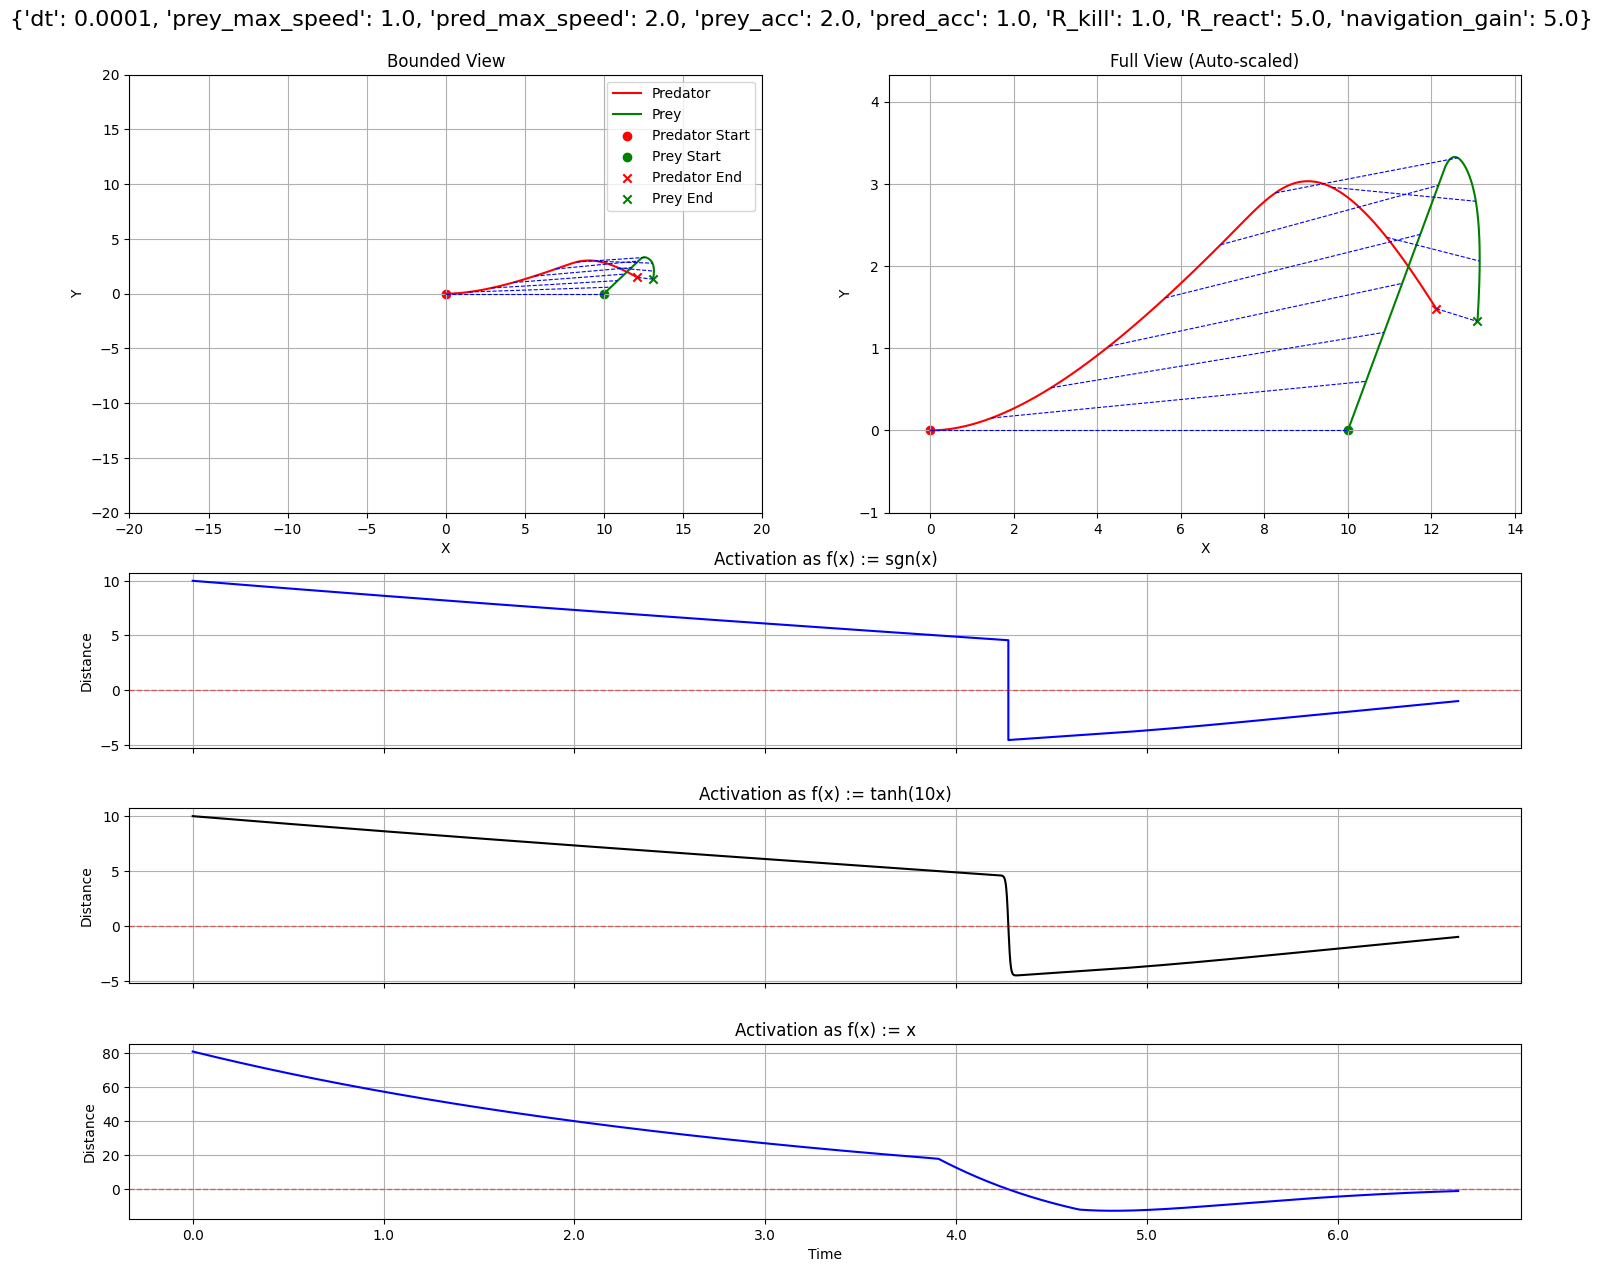
\includegraphics[width=0.45\textwidth]{figures/signed_distance.png}
          \label{fig:trajectory}
        \end{figure}

        We can notice a clear tradeoff between the regularity of the `Signed Distance Function' and its fidelity in representing both sign and distance, which depends on the activation. In fact, smoother approximations of the \textit{sign}function can provide more regular signed distance, at the cost of deviating from the pure form of sign $\times$ norm.

        We proceed by observing how initial conditions affect behaviour: we vary initial bearing, that is, the angle of the prey at the initialization, while fixing the predator's initial conditions. We then plot for reference both scaled and normalised plots of $(x,y)$ trajectories, showing the relative positions between prey and predator using isochrone lines. To complete the picture, we show the evolution of some relevant metrics over the run.

        \begin{figure}[H]
          \centering
          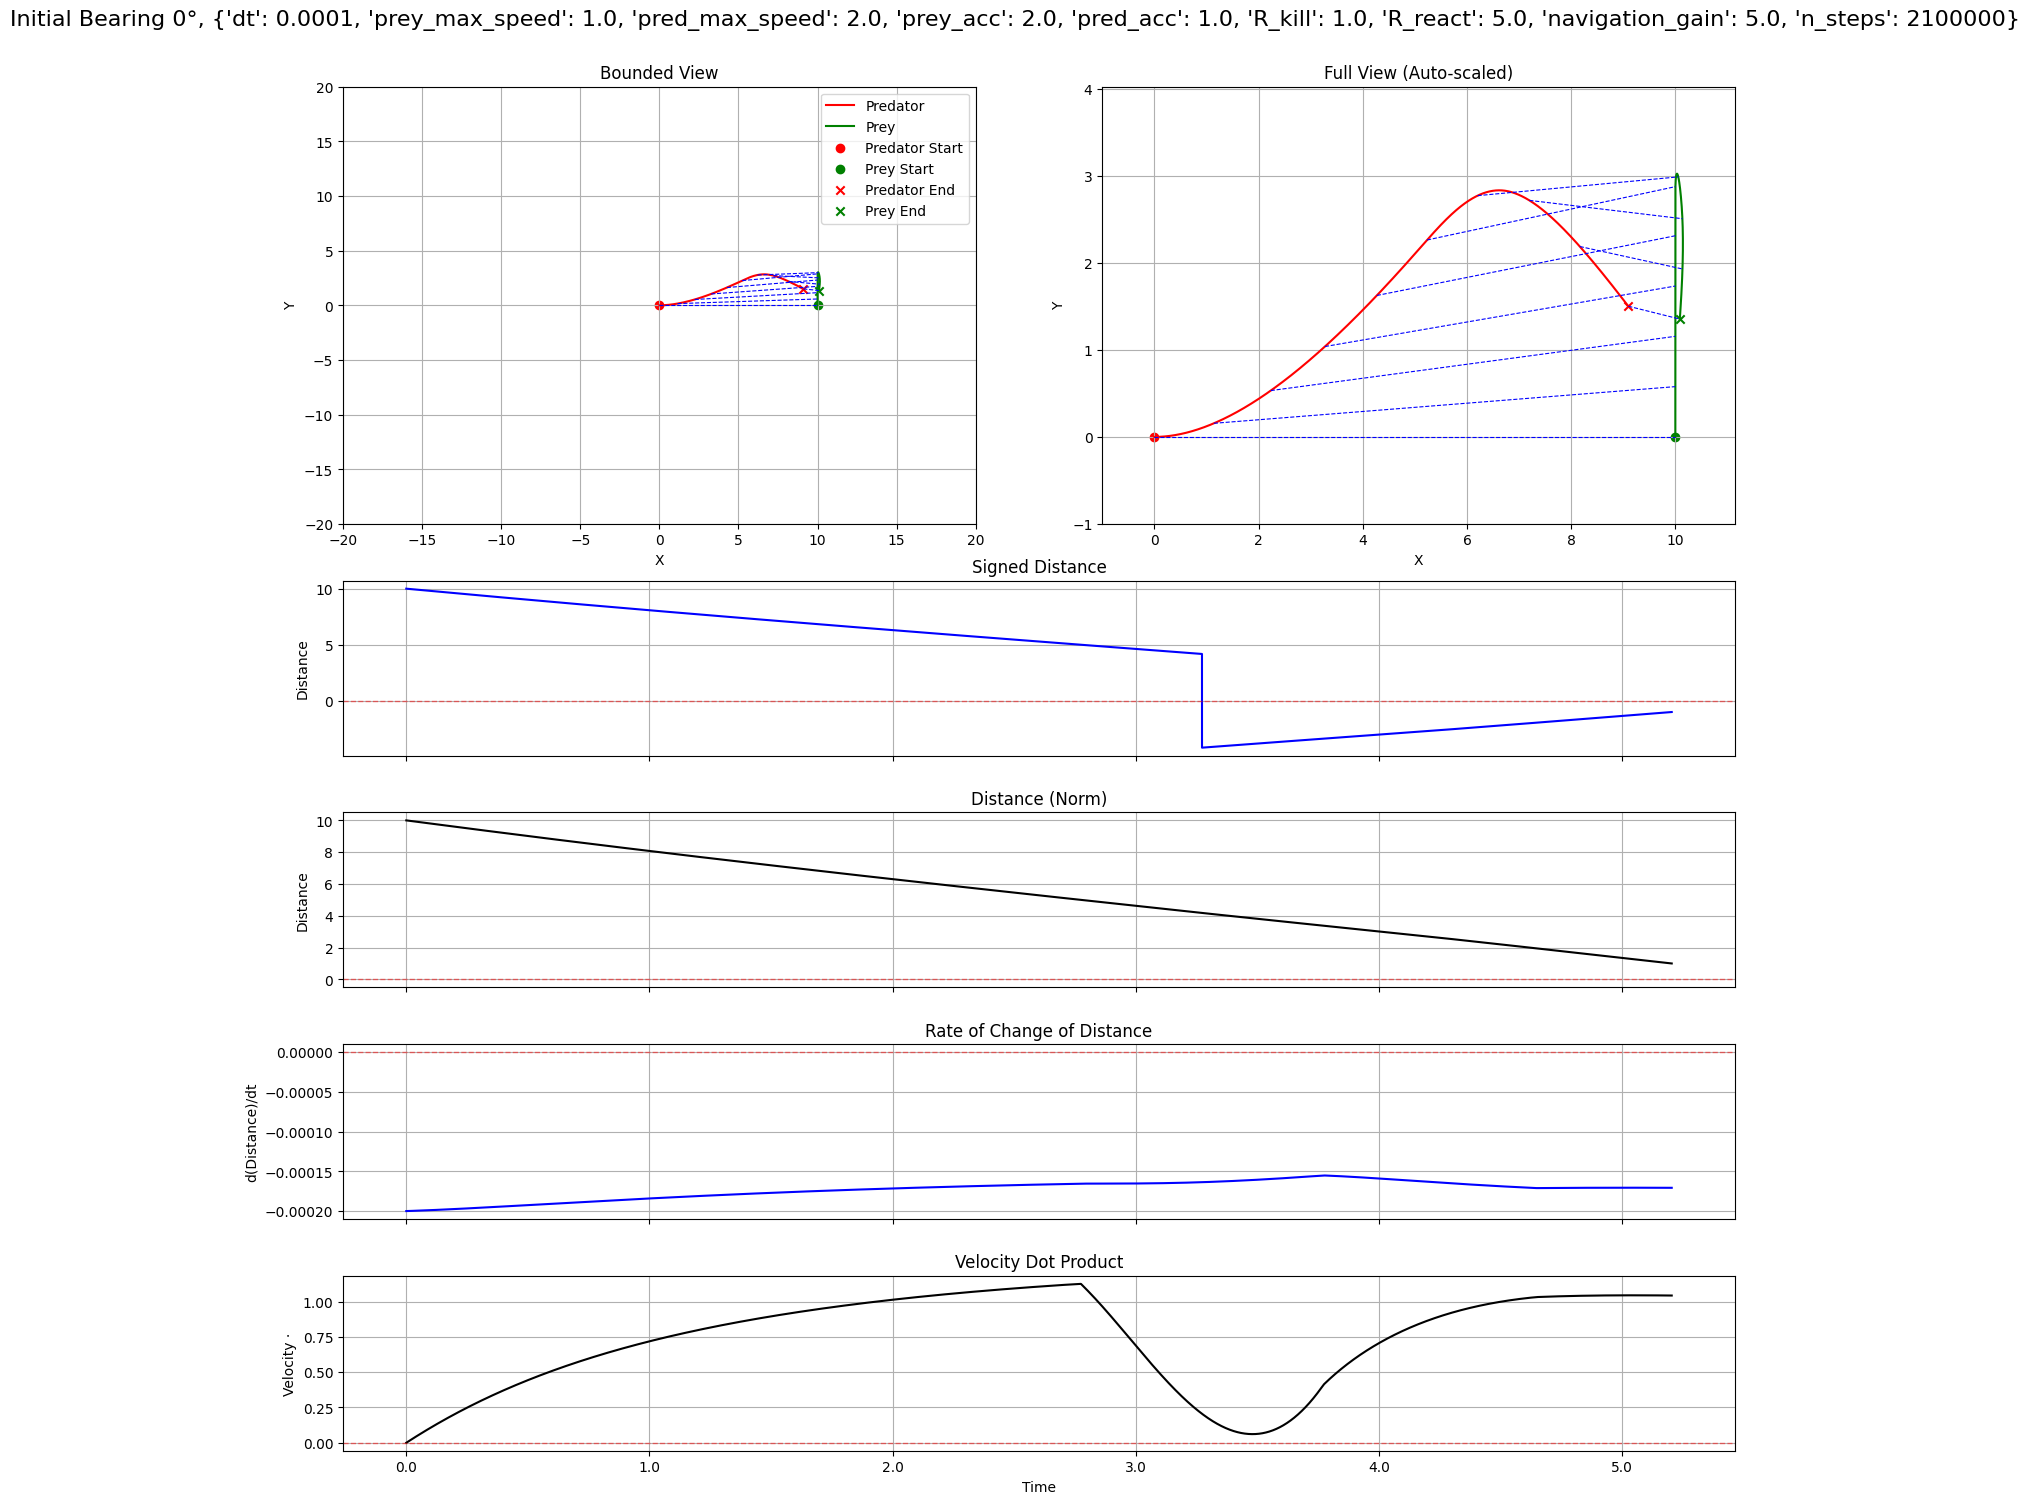
\includegraphics[width=0.45\textwidth]{figures/initial_bearing_120.png}
          \caption{Initial bearing of 120°}
          \label{fig:bear120}
        \end{figure}

        \begin{figure}[H]
          \centering
          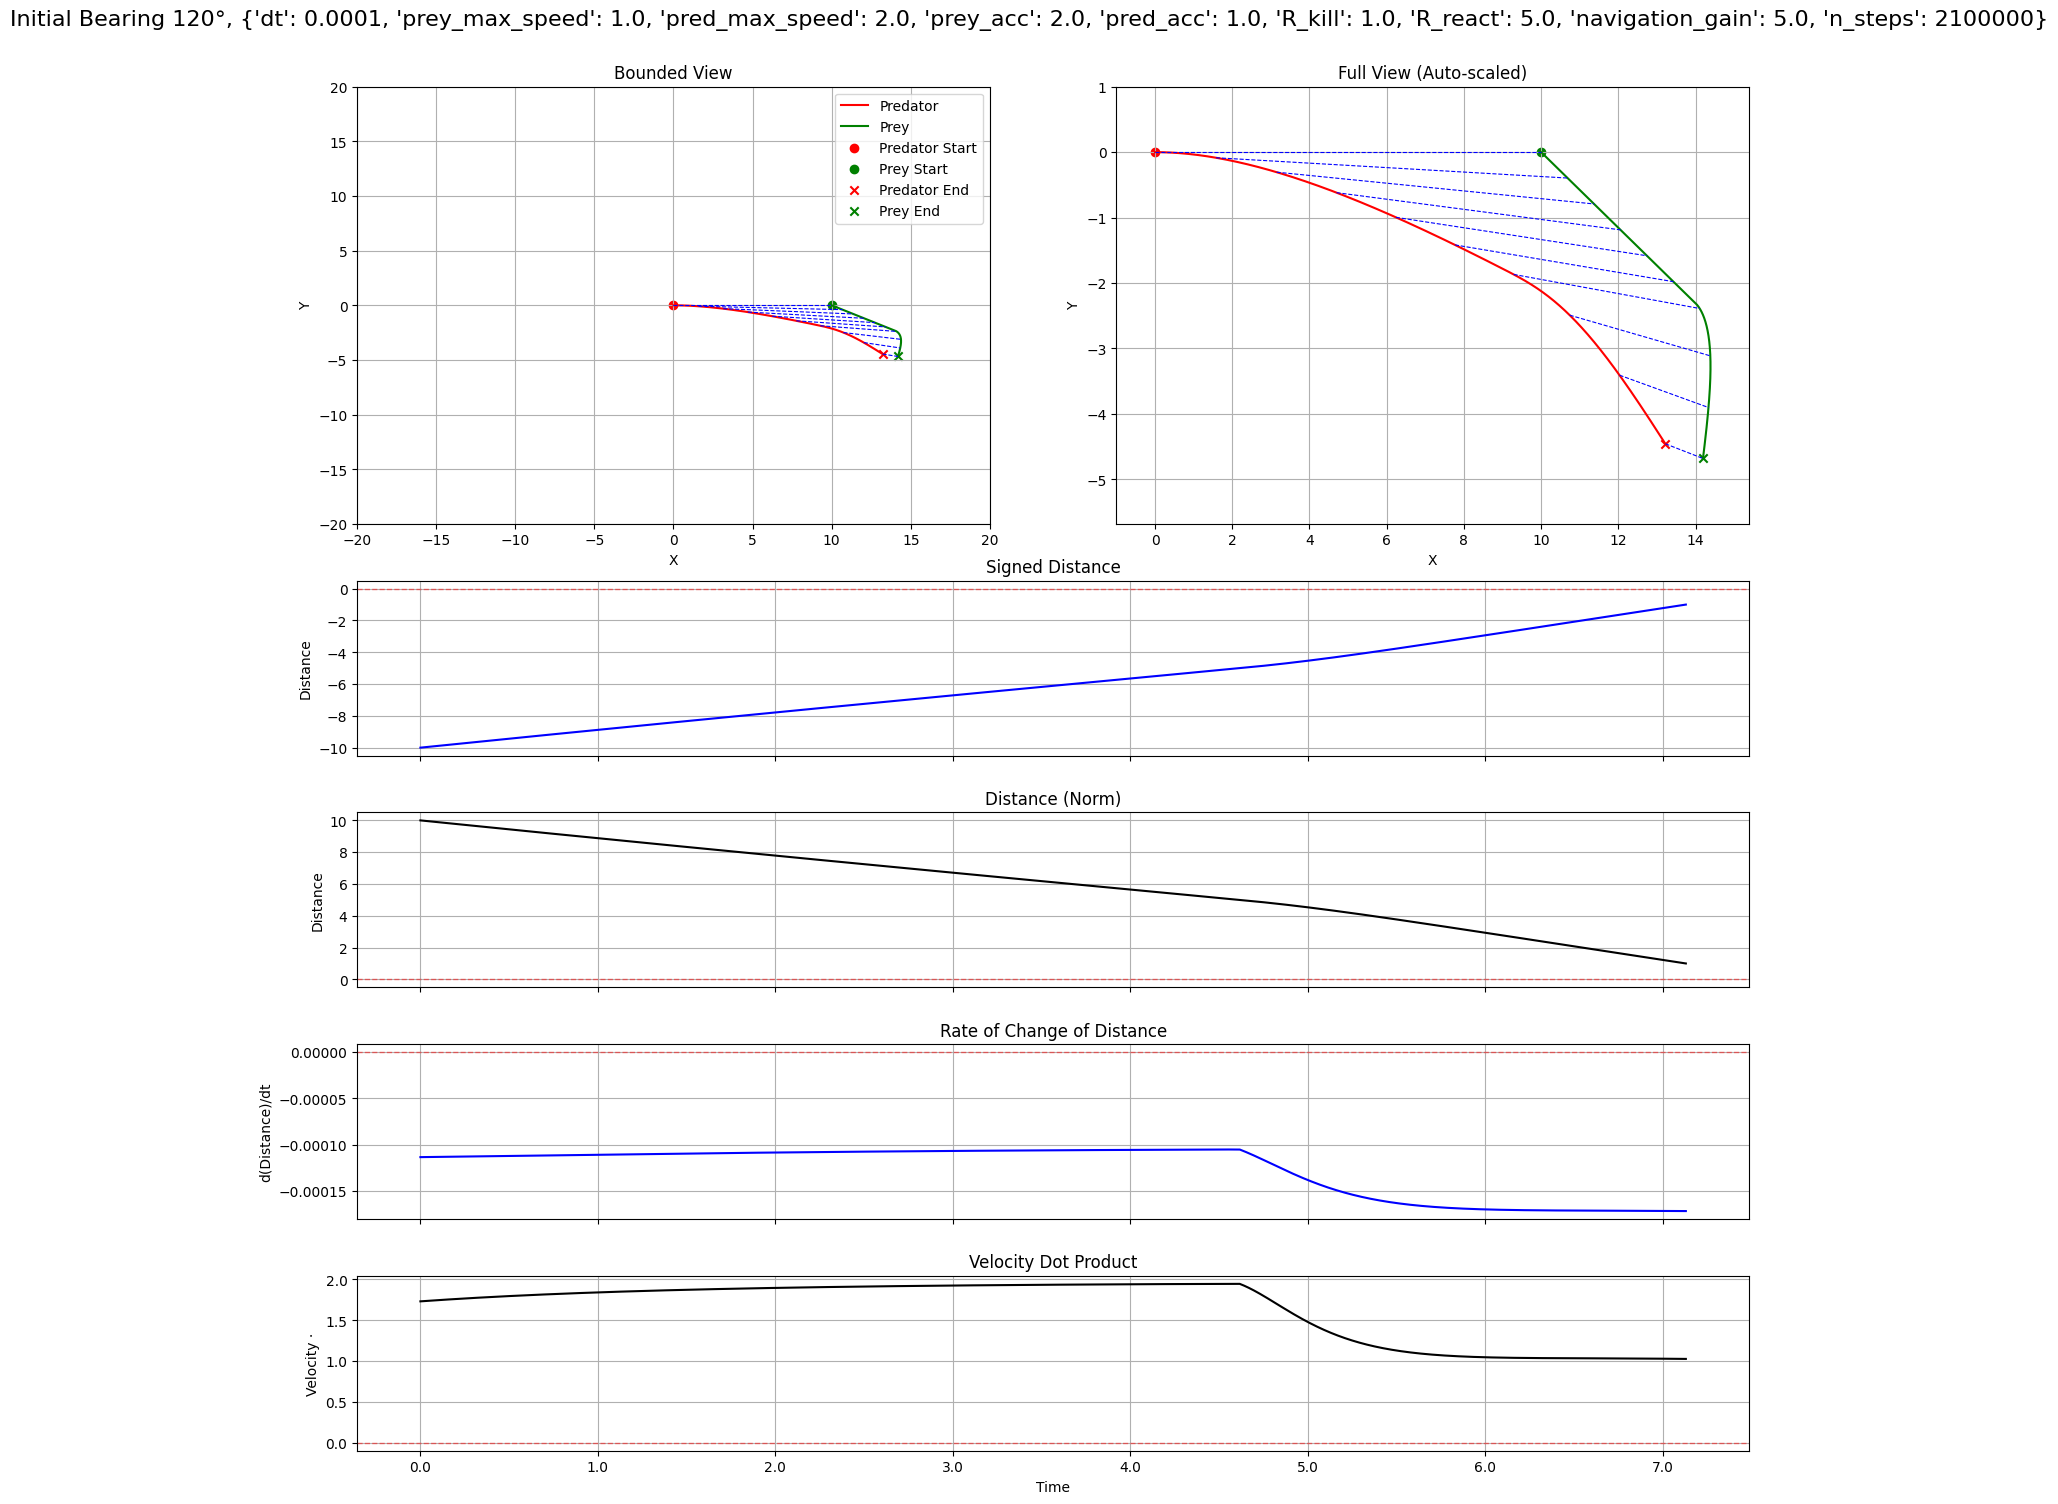
\includegraphics[width=0.45\textwidth]{figures/initial_bearing_240.png}
          \caption{Initial bearing of 240°}
          \label{fig:bear240}
        \end{figure}

        The presence of waves and suggests the need to use more advanced methods to understand the behavior. We use the Cosine Transform to estimate the natural frequency of the waves: this technique consists in decomposing the function into the cosine waves, which is the natural method to identify the "dominant" frequencies within a periodic function.

        To characterise the behaviour of the metrics in the trajectories, we use the Discrete Cosine Transform, which has a time complexity in the order of O(N*log(N)) of functions of length $N = 2^K$. As a philosophical assumption, we employ a window function to reduce the effect of initial and final behaviour in the wave, focusing on the behaviour over the run. This technique allows us to abstract from specific conditions, focusing only on the trajectory, since the cutoff is arbitrary, which leads to noise in the transformation.

        We plot the log-log Discrete Cosine Transform to study the results shown before: decomposing the signed distance for the previous three trajectories, we notice that the \textit{Hamming Window} performs better, producing narrower peakes, which is more aligned with the "Dirac Comb" shape predicted theoretically.
        \begin{figure}[H]
          \centering
          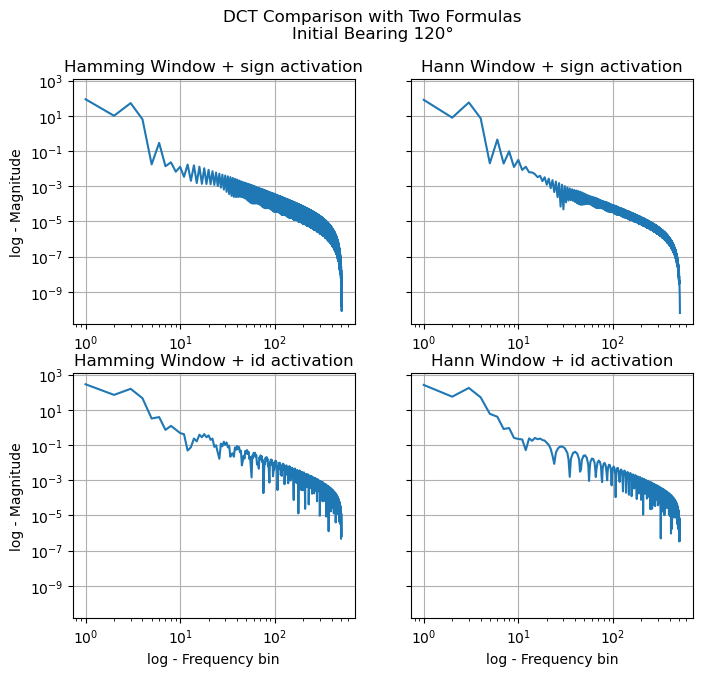
\includegraphics[width=0.45\textwidth]{figures/dct_120_loglog.png}
          \caption{DCT of first experiment with bearing of 120°}
          \label{fig:dct1}
        \end{figure}

        \begin{figure}[H]
          \centering
          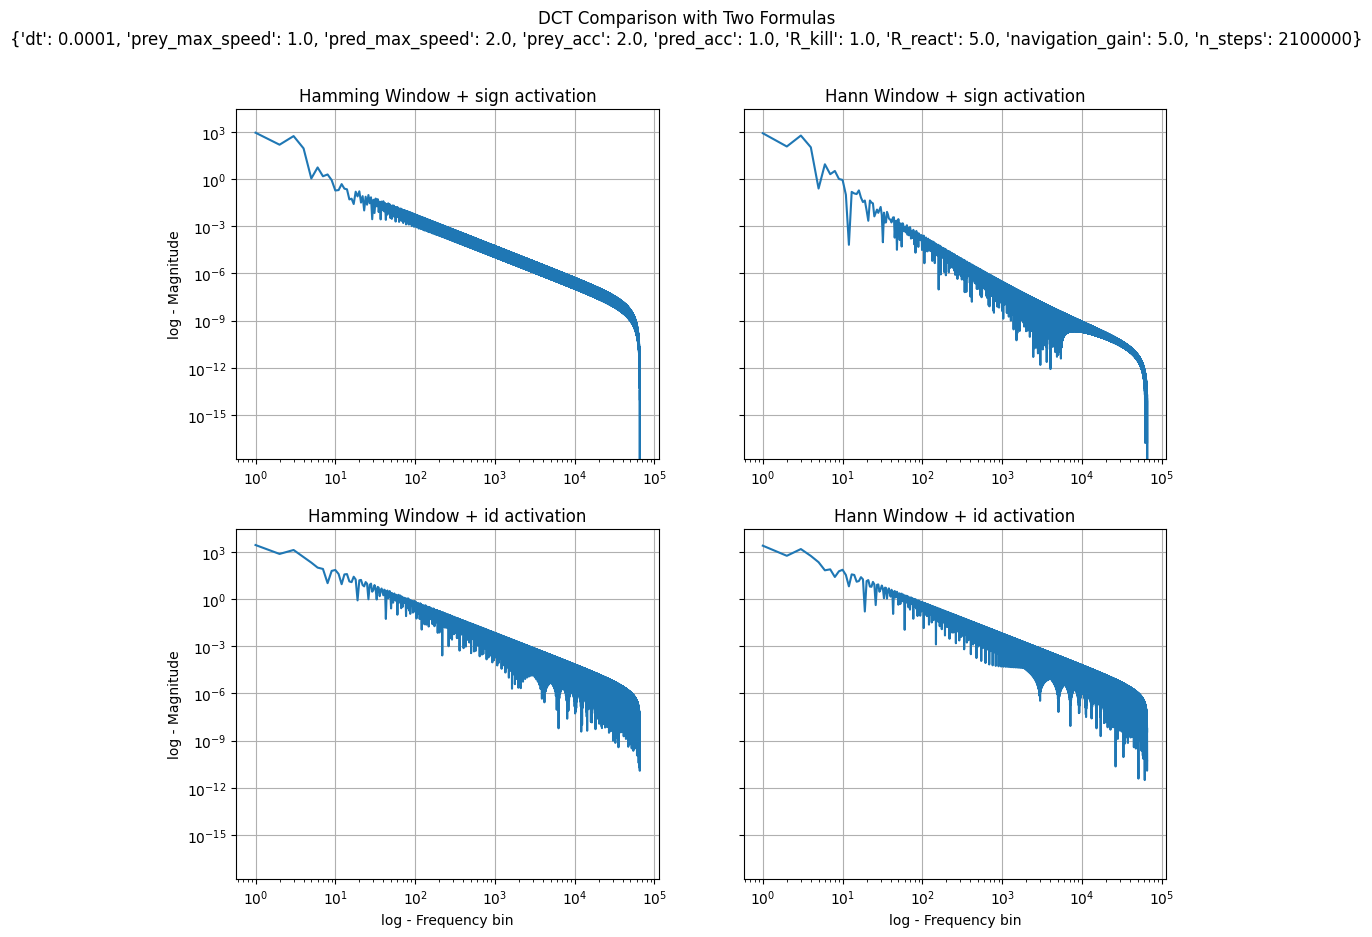
\includegraphics[width=0.45\textwidth]{figures/dct_240_loglog.png}
          \caption{DCT of second experiment with bearing of 120°}
          \label{fig:dct2}
        \end{figure}

        In the first plot, the `thumb' shapes of the cosine decomposition, may be informally understood by observing the behaviour of the similar function, such as $t(x) := \frac{2}{1+x^4}$, taken as a single peak in the decomposition. Evaluating the antitransform and observing the positive $x>0$ values, one recognises the behaviour and general shape of a damped oscillator, which is related to the behaviour of the first trajectory.

        \begin{figure}[H]
          \centering
          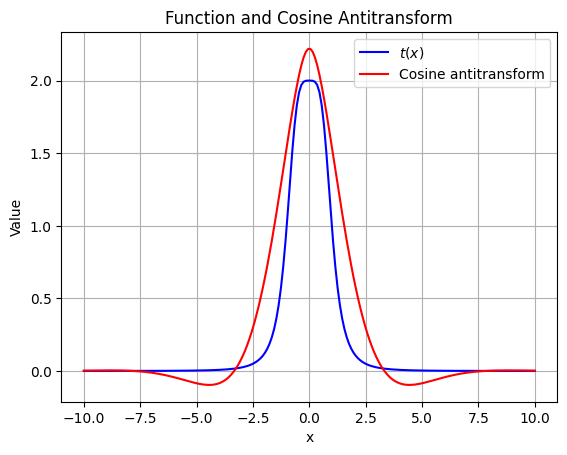
\includegraphics[width=0.45\textwidth]{figures/f_and_cos_antitr.png}
          \label{fig:antitransform}
        \end{figure}

        By observing the plots, we note three key characterizations of the waves, given their Cosine Transforms:
        \begin{itemize}
          \item \underline{Mean Distance}: the y-axis intercept shows the mean value of the function.
          \item \underline{Peak}: the Cosine Transform Identifies the key natural frequency of the way
          \item \underline{Noisy tail}: the higher end of the transform are particularly noisy, especially for waves with jumps.
        \end{itemize}

        We also observe the presence of noise, which may be attributed to the irregularities of the signed distance: in fact, when the identity is used as activation, the noise is reduced and the decay rate - the slope of the right tail - is stronger. It is clear that more regular waves produce sharper results. This is also apparent in the following plot, which display the cosine transform of the standard distance $d(x,y) := ||x(t)-y(t)||$, a more regular wave.

        On a final note, we conclude this section by noticing that `pure' frequency of the wave is easier to extract by only considering the distance (ie. the euclidean norm) in the space, at the cost of losing the qualitative aspect of the sign.

        \section{Phase Space Plots}
        We now consider ensemble plots of the prey-predator dynamics, to understand how acceleration and speed relate to pursuit-evasion effectiveness. To do this, we fix the starting conditions and vary continuously acceleration in the prey and maximal speed of the predator, while fixing all the other attributes.

        Although the following description does not paint a complete picture of the parameter space, studying a subset of their possible values highlights both an effective methodology and shows tangible behaviours that may emerge. In fact, the same tools shown in this investigation can be applied to evaluate specific parameter neighbourhoods in other values of the simulation.

        For matters of computational and memory efficiency, we proceed by computing the summary metrics for each trajectory at the end of each run, displaying the complete results only at the end through heatmaps.

        We use the following conditions to define the runs: we use a step size of 100 to interpolate a square range of $(v^\text{max}_y, a_x)$ values, where each combination corresponds to a run. We then plot different metrics for each run.

        \[
          \begin{aligned}
            &n_{\text{ticks}} = 100, \quad \Delta t = 0.0001,\quad t_{\text{max}} = 20,\quad n = 5 \\
            &\left\{
              \begin{aligned}
                &v_y \in [1, 10],\quad a_x \in [1, 10] \\
                &a^{\text{max}}_y = 1,\quad R_{\text{kill}} = 1 \\
                &v^{\text{max}}_x = 1,\quad R_{\text{react}} = 5
              \end{aligned}
              \right.
            \end{aligned}
          \]

          For practical reasons, we impose a $t_{\text{max}}$ term, which bounds the maximum duration of the trajectory, to discard trajectories which never converge.

          \begin{figure}[H]
            \centering
            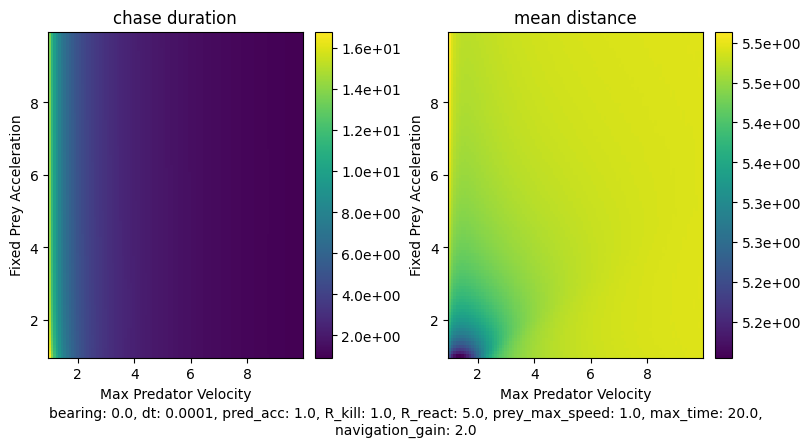
\includegraphics[width=0.45\textwidth]{figures/phase_duration_distance.png}
            \label{fig:phaseplot1}
          \end{figure}

          As a preliminary step, we observe chase duration and confirm that, as expected, reducing the predator's `max velocity` leads to longer chases, up to never catching the prey. This is clear from the value, which achieves the maximum time. On the other hand, `predator velocity` values greater than $v_x^{\text{max}}=2$ seem to induce a shift in behaviour, with predators catching up in approximately in time $2.5 < t_{\text{max}} = 20$.

          In an inverse manner, average distance is uniform for $v_x^{\text{max}}>2$. We finally observe that similarly matched prey and predator, with both acceleration and speed low and equal, tend to remain close over the chase, which is clear from the lower-left corner in the mean-distance graph.

          In few words, chases are short and successful for all prey accelerations, assuming the predator has high enough speed.

          \begin{figure}[H]
            \centering
            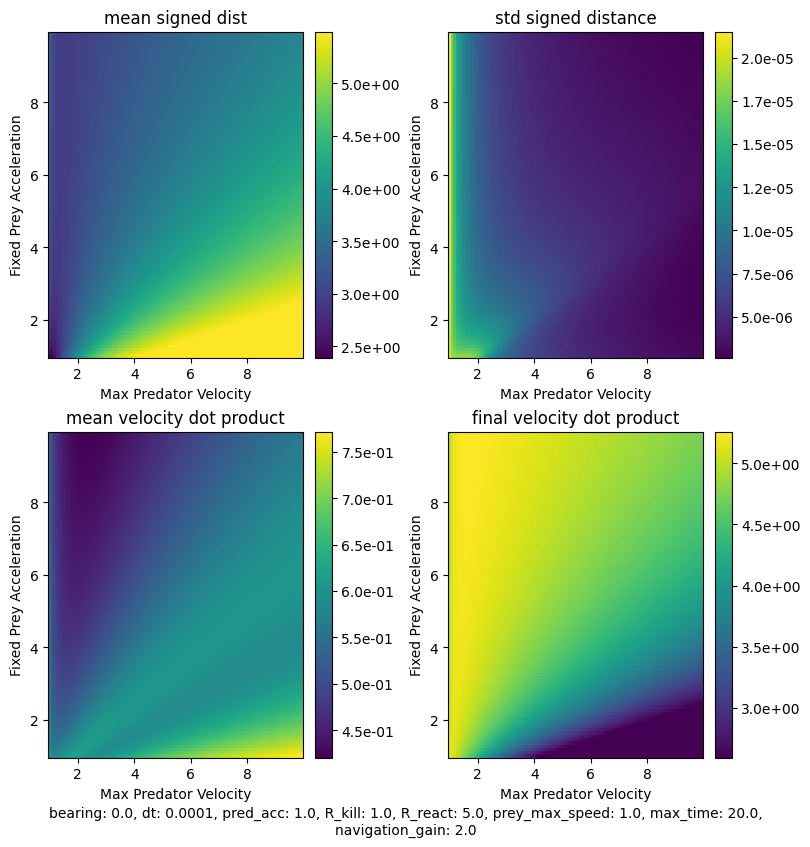
\includegraphics[width=0.45\textwidth]{figures/phase_avg_dist_dot.png}
            \label{fig:phaseplot2}
          \end{figure}

          Mean distance and the dot product of the velocities highlight another qualitative difference in behaviour: for approximately $a^{\text{max}}_x > 0.5\cdot v^{\text{max}}_y - 1$, we observe both higher average alignment between the velocities and a lower final alignment. This behaviour also corresponds to a higher average signed distance value. In these runs, the predator catches up to the prey from one side, but intercepts it at a sharper angle of attack. Interestingly, the opposite effect happens when the proportions are reflected, producing a lower mean alignment over the chase but higher alignment at the end, which highlights that the predator chases the prey from afar, converging to it near the end. Clearly, depending on the relation between predator velocity and prey acceleration, trajectories will either be aligned over the run or at the intercept.

          Consistent with these observations, the boundary of runs that lead to a sharper final angle of attack is notable from the point of view of the rate of change of distance, which has high variability over the run. This is consistent with an expected `phase change` of the system.

          \begin{figure}[H]
            \centering
            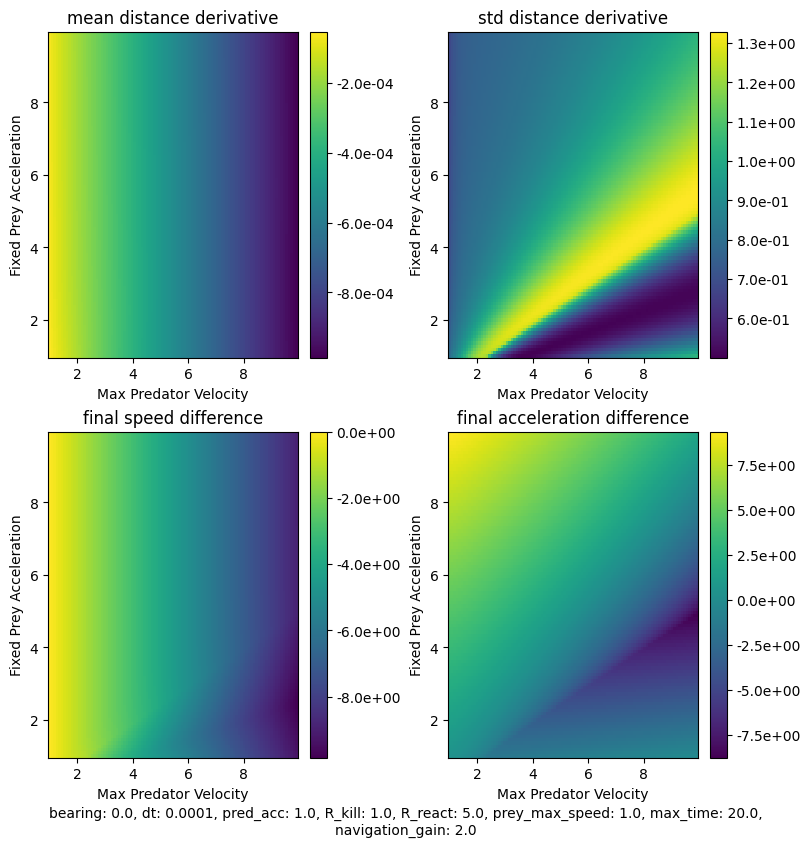
\includegraphics[width=0.45\textwidth]{figures/phase_derivative_dist.png}
            \label{fig:phaseplot3}
          \end{figure}

          As a final remark, we observe that distance always decreases over the runs, with a faster initial rate at the beginning, regardless of prey acceleration, and lowers near the end. Similarly, the final difference between the speeds decreases, though it generally remains negative, as the predator is faster.
          \section{Conclusion}
          Even when it is reduced to simple and deterministic decision rules for both prey and predator in $\mathbb{R}^2$, the \textit{Homicidal Chauffeur Problem} can exhibits a rich variety of behaviours. In our investigation, we picked right-angle evasion for the prey and Proportional Navigation for the predator; after defining the setting and assumptions, we identified relevant metrics for studying the trajectories: signed and unsigned distances are qualitative indicators of the efficiency of the chase, while the dot product between the velocities highlights alignment in direction between the agents. We compared variations of signed distances through an activation function and applied the cosine transform to study single trajectories, concluding that the most informative log-log plot may be produced through a Hamming window function applied to the positive distance metric. Finally, we picked a region of the parameter space and for fixed initial conditions we varied predator maximum speed and prey acceleration. We identified a two roughly symmetric basins of behaviours, in which predators, if fast enough in relation to the prey's acceleration, chase it in parallel but intercept it at a steep angle of attack, while the opposite phenomenon occurs in the reverse.

          \begin{thebibliography}{99}
            \bibitem{DCT} The discrete cosine transform and JPEG. (2022, March 22). ESE 224 Signal and Information Processing. \url{https://ese2240.seas.upenn.edu/lab-9-the-discrete-cosine-transform-and-jpeg/}. Accessed 26 May 2025
            \bibitem{loglog} Log–log plot. (2024, November 25). Wikipedia. Wikimedia Foundation. \url{https://en.wikipedia.org/wiki/Log%E2%80%93log_plot}. Accessed 26 May 2025
              \bibitem{Isaacs51} R. Isaacs, \emph{Games of Pursuit: P-257}. Contributions to the Theory of Games, P (Rand Corporation), Rand Corporation, 17 November 1951, 28 pp.
            \end{thebibliography}
            \end{document}
